
\documentclass[xcolor=dvipsnames]{beamer} 
\usecolortheme[named=Blue]{structure} 
\usetheme[height=10.5mm]{Rochester} 
\setbeamertemplate{items}[ball] 
\setbeamertemplate{blocks}[rounded][shadow=true] 
\setbeamertemplate{navigation symbols}{} 
\usepackage{bm}
\usepackage{listings}
\usepackage{rotating}
\usepackage{graphicx}
\usepackage{multirow}
\usepackage{hyperref}
\usepackage{textcomp}
\usepackage{upquote}
\usepackage[absolute,overlay]{textpos}
\newenvironment{reference}[2]{%
  \begin{textblock*}{\textwidth}(#1,#2)
      \footnotesize\it\bgroup\color{red!50!black}}{\egroup\end{textblock*}}
%\graphicspath{ {/home/ben/PhD/Armidale_Updates/2014_03_14/Figures/} }
\begin{document}

%%% New plan for this module:
%%% we all use Git on the command line and view GitHub in our web browsers
%%% clone and commit via HTTPS
%%% Workflow plan:
%%%
%%% Create repo in web browser
%%% Authenticate on cmd line
%%% Clone
%%% Add files
%%% Edit
%%% git add
%%% git commit
%%% branch and revert to previous version with check out


%%% Getting on the command line in various OS's

%%% MS Windows -> Start Menue -> Powershell
%%% Mac OS -> Finder -> terminal
%%% GNU+Linux users -> application launcher (will vary depending on GUI) -> terminal 


\begin{frame} %1
% \frametitle{Addressing Common Challenges in Spatial Modeling of Ecologies and Environments}
\begin{center}
\textbf{\huge Version Control with Git}\\
\end{center}

\begin{figure}
%\includegraphics[width = 0.35\textwidth]{/home/ben/Intro_to_R/GitHub_Slides_Source/Images/GitHub-Mark-120px-plus.png}
\begin{columns}

\begin{column}{3.3cm}
\begin{center}
\begin{figure}

\includegraphics[width = 0.9\textwidth]{/home/ben/Intro_to_R/Introductory_Slides_Source/Images/R_logo.png}
\end{figure}
\end{center}
\end{column} 

\begin{column}{3.3cm}
\begin{center}
\begin{figure}

\includegraphics[width = 0.9\textwidth]{/home/ben/Intro_to_R/GitHub_Slides_Source/Images/Git-Icon-1788C.pdf}
\end{figure}
\end{center}
\end{column} 

\begin{column}{3.3cm}
\begin{center}
\begin{figure}

\includegraphics[width = 0.9\textwidth]{/home/ben/Intro_to_R/GitHub_Slides_Source/Images/GitHub-Mark_Big.pdf}
\end{figure}
\end{center}
\end{column} 

\end{columns}
\end{figure}

\small Ben R. Fitzpatrick\\
\tiny PhD Candidate, Statistical Science, Mathematical Sciences School, Queensland University of Technology
\newline
\begin{columns}
\begin{column}{3cm}
\tiny 0000-0003-1916-0939
\end{column}
\begin{column}{3cm}
\tiny github.com/brfitzpatrick/
\end{column}
\begin{column}{3cm}
\tiny @benrfitzpatrick
\end{column}
\end{columns}
\end{frame}


\begin{frame} 
\frametitle{Plan for this Module - Part 1}
\begin{block}{Solo Version Control}
\begin{itemize}
\item Set up Git on your laptops to communicate with the GitHub servers
\item Create a local `clone' of a remote repository
\item Make some changes to your local copy of the files
\item commit these changes to the git version control system
\item push these changes to your repository
\item make some more changes
\item revert to a previous version of the file
\end{itemize}
\end{block}
\end{frame}

\begin{frame} 
\frametitle{Plan for this Module - Part 2}

\begin{block}{Collaborating with Git \& GitHub}
\begin{itemize}
\item fork
\item branch 
\item edit
\item commit
\item pull request
\item merge
\end{itemize}
\end{block}

\end{frame}

\begin{frame}
\frametitle{Version Control Software}
Have you ever put numbers or dates at the end of a file name to keep different versions of it? 
\begin{itemize} 
\item If yes then you have already used version control!
\newline
\newline
\end{itemize}

Have you ever used track changes and comments to take turns editing a  MS Word document with one or more others?
\begin{itemize}
\item If yes then you have collaboratively edited a file!
\newline
\newline
\end{itemize}

Version Control Software: 
\begin{itemize} 
\item formalizes these concepts
\item can do a lot of the organisational work for you
\item makes reverting to previous versions without losing work easy 
\end{itemize}
 
\end{frame}

\begin{frame}
\frametitle{Version Control when Working Alone}
Even if you are not collaborating with anyone on a particular file version control can still be very useful
You essentially have a time stamped undo button which will allow you to go review or revert to previous versions of the file
you can even make multiple child versions fo the same file say for different audiences or to trial different orders and styles in which to write a report or program
\end{frame}


\begin{frame}
\frametitle{Version Control when Collaborating}
Greatly simplifies your life
Control over which changes different contributers make get added to the definitive version of a file
support for file to split into two child copies which can then be edited towards very different end points but still having the option to systematically recombine them at any stage

\end{frame}

\begin{frame}
\frametitle{Why Git?}

Git is free and open source
\newline
\newline
Git is available for most operating systems
\newline
\newline
\begin{block}{Major Online Code Hosting Services Support Git:}
\begin{itemize}
\item GitHub \& BitBucket are the popular code hosting choices these days
\item GitHub \& BitBucket both allow code management with Git
\item GitHub \& BitBucket both have free code hosting options
\end{itemize}
\end{block}

Git is Distributed and Fast

\tiny $^1$ Google Code will close in 2016 as they have deemed it is no longer necessary given success of BitBucket and GitHub

\end{frame}



\begin{frame} 
\frametitle{Git is Distributed Version Control}
Every contributor has a copy of the entire database ( all revisions of all files)
two contributors can both work on the files in their copy of the database independently then their combined modifications can be merged systematically
\end{frame} 

\begin{frame}
\frametitle{Why Git on the Command Line?}
Makes discrete components of the workflow obvious this in turn will enable you to migrate easily to one of the many GUIs
\newline
\newline
The workflows we will practise today will work exactly the same way on MS Windows, MacOS and GNU+Linux
\newline
\newline
By this stage we have been using a command line interface for 1.5 days to interact with the R program it's time to take it to the next level
\end{frame}

\begin{frame}
\frametitle{Creating a Repository on the GitHub Servers}
\framesubtitle{Log into the GitHub Web Service}
\begin{center}
\begin{figure}
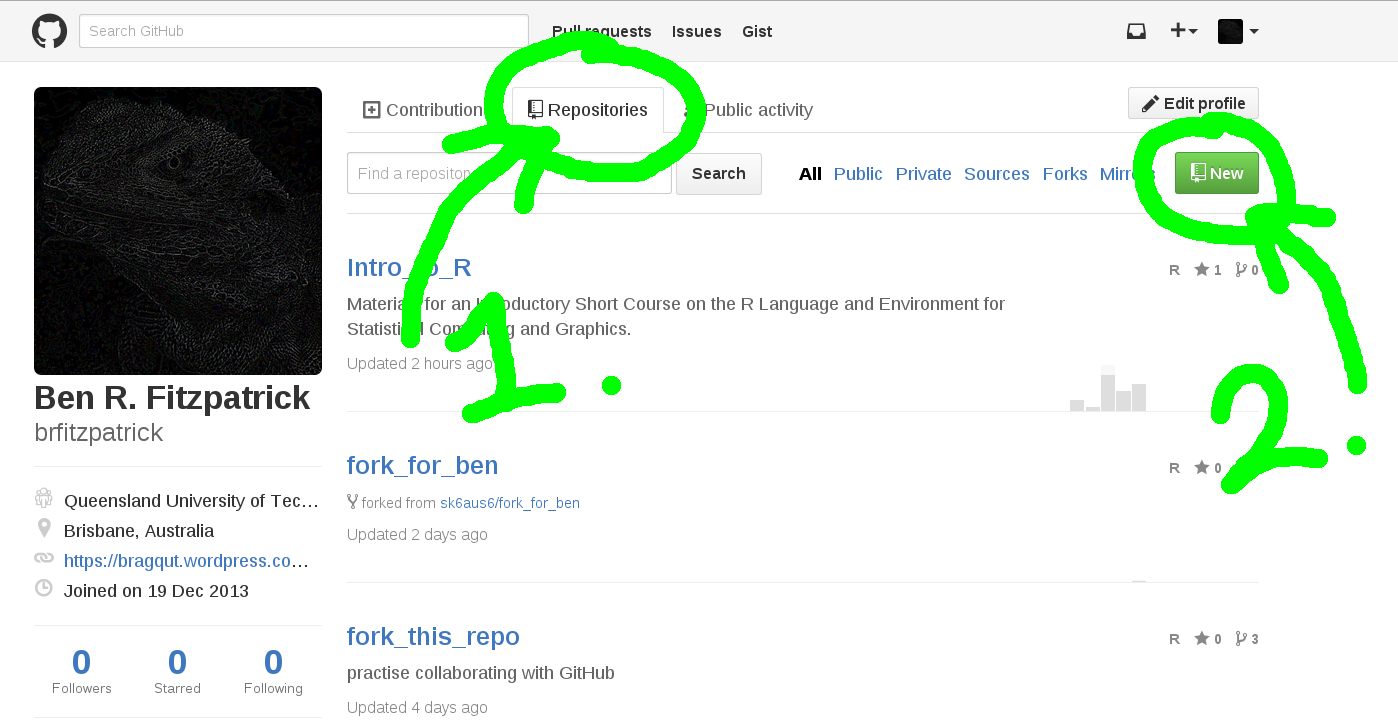
\includegraphics[width = \textwidth]{/home/ben/Intro_to_R/GitHub_Slides_Source/Images/New_Repo_1.png}
\end{figure}
\end{center}
\end{frame}

\begin{frame}
\frametitle{Creating a Repository on the GitHub Servers}
\framesubtitle{Complete the Details}
\begin{center}
\begin{figure}
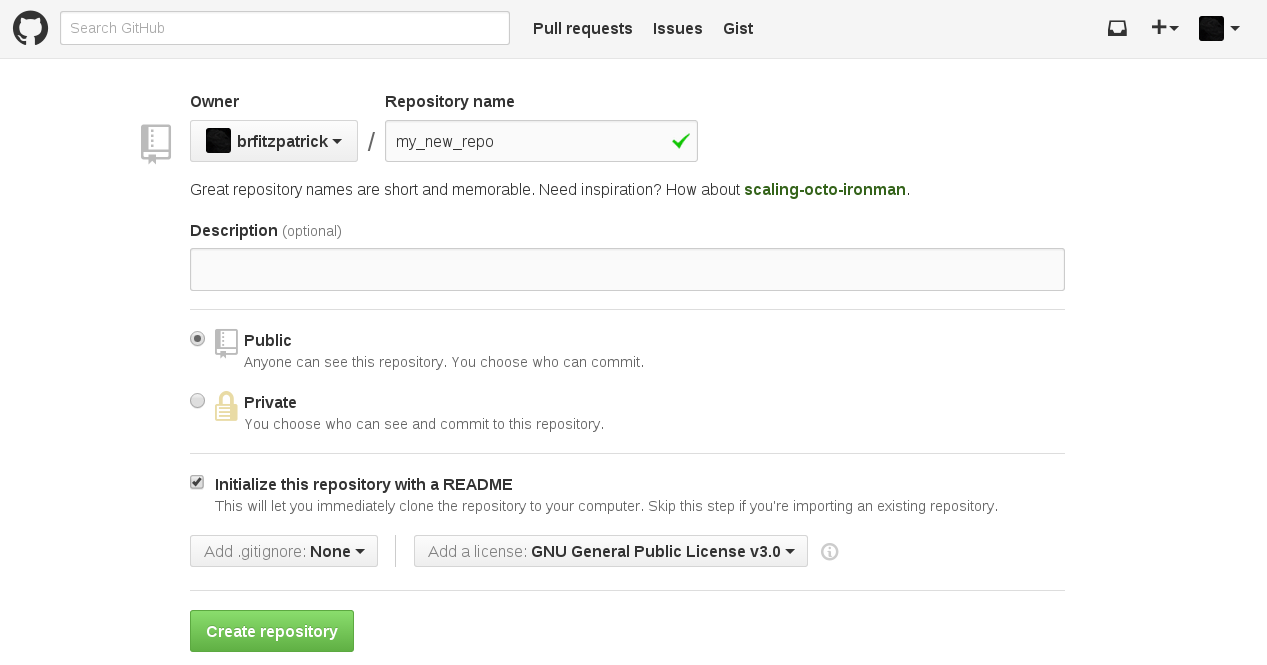
\includegraphics[width = \textwidth]{/home/ben/Intro_to_R/GitHub_Slides_Source/Images/New_Repo_2.png}
\end{figure}
\end{center}
\end{frame}

\begin{frame}
\frametitle{Creating a Repository on the GitHub Servers}
\framesubtitle{View your New Repository}
\begin{center}
\begin{figure}
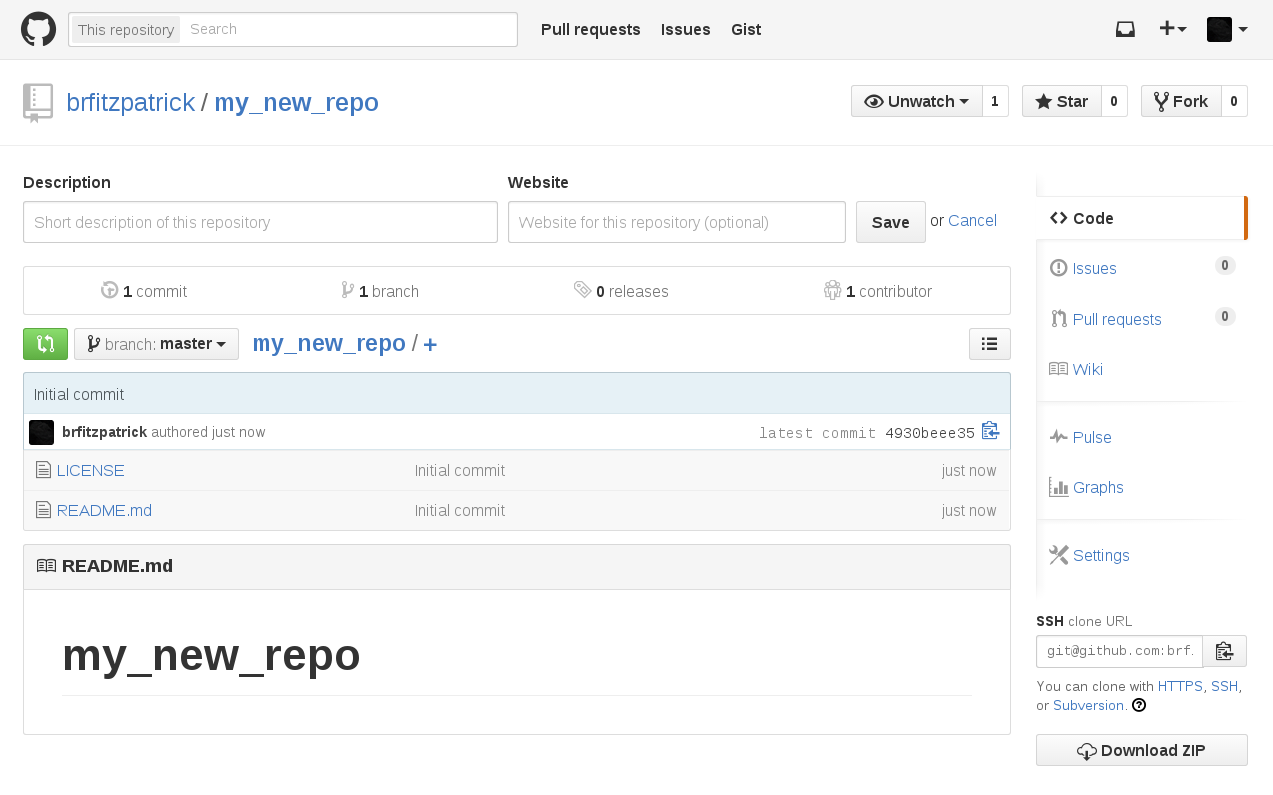
\includegraphics[width = \textwidth]{/home/ben/Intro_to_R/GitHub_Slides_Source/Images/New_Repo_3.png}
\end{figure}
\end{center}
\end{frame}

\begin{frame}
\frametitle{Next - to clone your repository to the hard drive of your laptop}
Create a folder to store your Git Repositories on your Hard Drive

\end{frame}


\begin{frame}
\frametitle{Accessing a command line interface in your OS of choice}

\begin{columns}

\begin{column}{3.3cm}

\begin{center}
MS Windows\\
Open a `PowerShell'

\begin{figure}
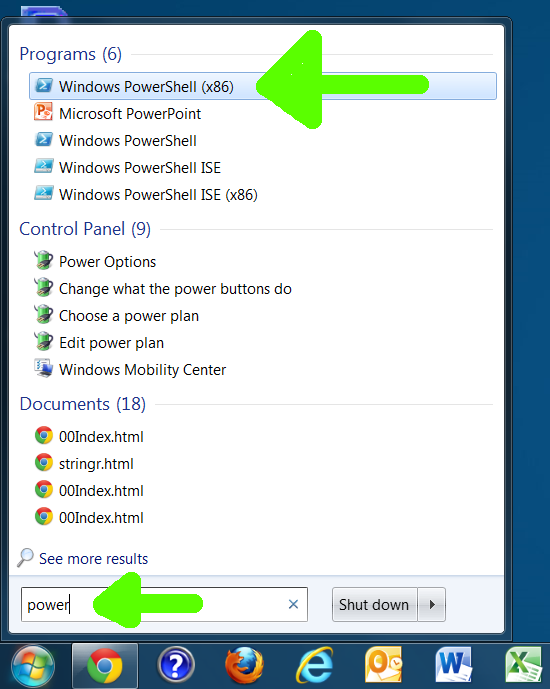
\includegraphics[width = \textwidth]{/home/ben/Intro_to_R/GitHub_Slides_Source/Images/Git_on_MS_Windows_Powershell/Powershell.png}
\end{figure}

\end{center}

\end{column} 

\begin{column}{3.3cm}
Mac OS X \& later\\
Open a `Terminal'
%\begin{center}
%\begin{figure}
%\includegraphics[width = 0.9\textwidth]{} %% insert MacOS Screenshot here
%\end{figure}
%\end{center}
\end{column} 

\begin{column}{3.3cm}

\begin{center}
GNU+Linux\\
Open a `Terminal'

\begin{figure}
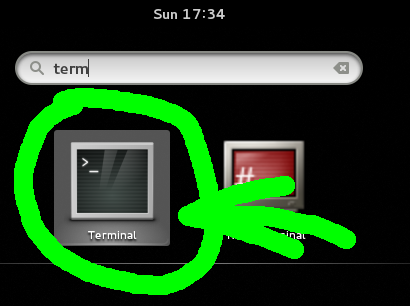
\includegraphics[width = \textwidth]{/home/ben/Intro_to_R/GitHub_Slides_Source/Images/Git_on_GNU_Linux_Terminal/Launch_Terminal.png}
\end{figure}

\end{center}

\end{column} 

\end{columns}
\end{frame}

\begin{frame}
\frametitle{Copy HTTPS URL to use when cloning repository}
\begin{center}
\begin{figure}
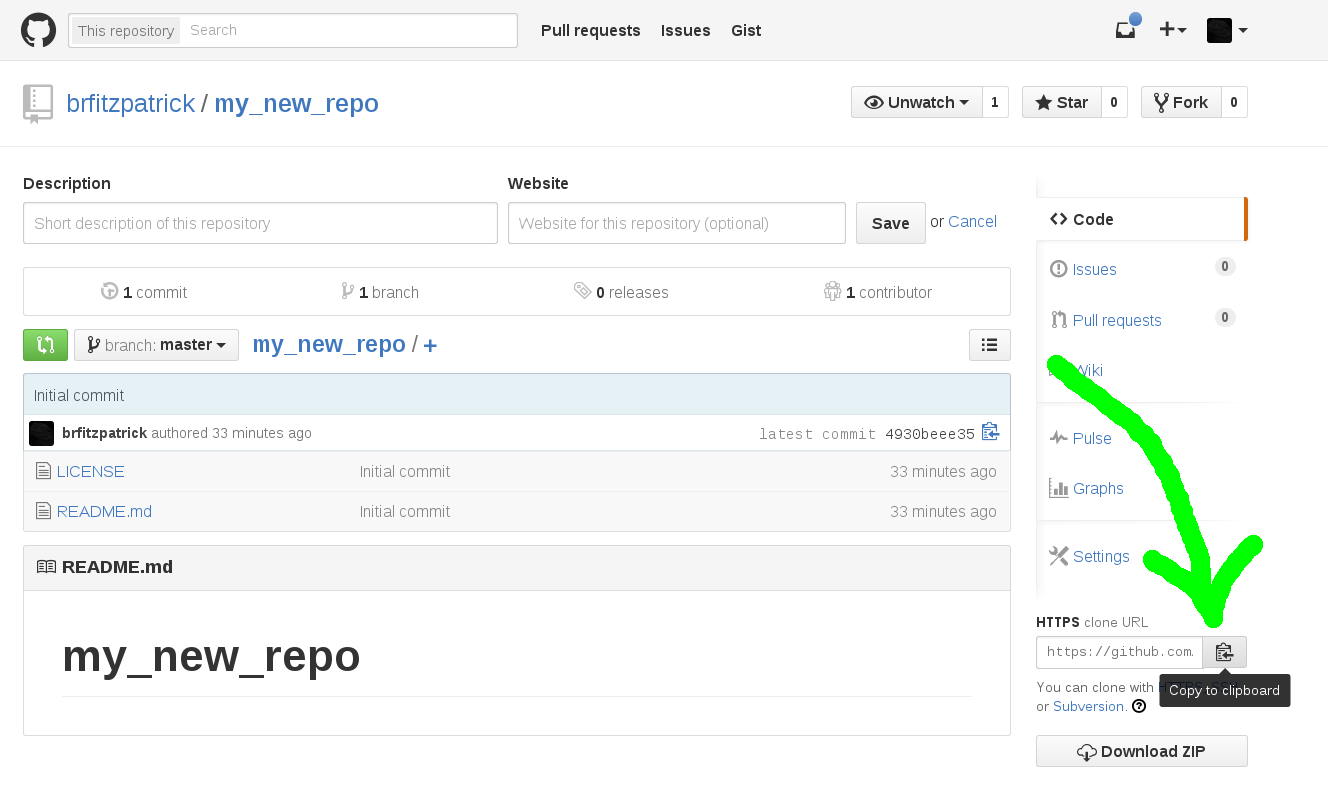
\includegraphics[width = \textwidth]{/home/ben/Intro_to_R/GitHub_Slides_Source/Images/Clone_Repo_1.png}
\end{figure}
\end{center}
\end{frame}

\begin{frame}[fragile]
\frametitle{Configuring Git for the first time}
\begin{block}{All Users}
\begin{lstlisting}
> git config --global user.name "Your Name"
> git config --global user.email you@mail.com
\end{lstlisting}
\end{block}
\end{frame}


\begin{frame}[fragile]
\frametitle{Cloning Your Repository from the GitHub Servers}

\begin{block}{Powershell Users}
\begin{lstlisting}
> C:
> cd C:\Users\username\Document\GitHub_Repos\
> dir 
\end{lstlisting}
\end{block}

\begin{block}{Terminal Users}
\begin{lstlisting}
> cd /home/ben/Documents/GitHub_Repos
> ls 
\end{lstlisting}
\end{block}
\end{frame}

\begin{frame}[fragile]
\frametitle{Clone Git Repository from the GitHub Servers to Your Hard drive}
Use the HTTPS URL you copied earlier!\\
\begin{center}
\begin{figure}
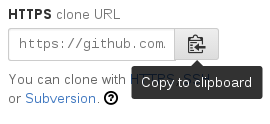
\includegraphics[width = 0.5\textwidth]{/home/ben/Intro_to_R/GitHub_Slides_Source/Images/HTTPS_Clone.png}
\end{figure}
\end{center}
Make sure the terminal/powershell has the working directory where you want to clone the repository
\begin{block}{All Users}
\begin{lstlisting}
> git clone https://github.com/.../my_new_repo.git
> cd ./my_new_repo/
> ls
> git status
\end{lstlisting}
\end{block}
\end{frame}

\end{document}

\begin{frame} 
\frametitle{Git}
\framesubtitle{The Three States of Files in a Git Tracked Directory}
Files in a directory which you are version controlling with Git can exist in one of three states:
\begin{itemize}
\item \textbf{committed} data stored in the database for the associted repository
\item \textbf{modified} local copy of a file (in your working directory) is different to the most recent version of that file stored in the database for the associted repository i.e. you have changed something but not comitted the changes (yet)
\item \textbf{staged} the local copy of a file which you have modified is marked to be added to the database in the next commit snapshot you send to the database

\end{itemize}

\end{frame}

\begin{frame} 
\frametitle{Git}
\framesubtitle{Basic Git Workflow}

\begin{itemize}
\item you modify files in your local copy of the repository
\item you stage these modified files ready to be committed to the database for the repository
\item you perform a commit which takes the files as they were when staged and stores a snapshot of them in the database for the repository
\end{itemize}

\begin{frame} 
\frametitle{Git}
\framesubtitle{Basic Git Workflow}

\end{frame}

\begin{frame} 
\frametitle{Git}
\framesubtitle{Undoing things}

\end{frame}


\begin{frame}
\frametitle{Branching}

'Branching means you diverge from the main line of development and continue to do work without messing with that main line.'

Every project starts with the default `master' branch
you can then make a new branch e.g. a `testing' branch which will initially be the same as the `master' branch at the point in time at which you create it
you switch to another branch by `checking out' that branch
you can then commit changes to this branch without alterning the `master' branch i.e. you could develop some new feature without risking breaking the functionality of the master branch while you do so
once your feel your work on the a branch is complete you can `merge' your `testing' branch with the `master' branch

branching allows for collaboration, various contributors can all make their own branches of the repository then submit their changes to the repository owner for merging into the master branch - git provided powerful tools for managing these merges and resolving merge conflicts

\end{frame}


\begin{frame}
\frametitle{Forking}
Fork a repository
Use the Sync button in Windows/MacOS client to get new changes from server (and submit any changes you have made)
\end{frame}



\begin{frame}
\frametitle{Create a Repository, Add Some Files}
\begin{itemize}
\item Log into your Github account
\item Click the Repositories Tab
\item Click the 'New' button (it's green)
\item name your repository
\item make it public (we can do a private one later)
\item intialize repository with a README
\item add a license GPL or MIT are easy FOSS licenses
\item clone the repository to your hard drive
\item add a file to your local clone of the repository
\item commit it to the repository
\item push your changes to the remote repository
\end{itemize}
\end{frame}

\begin{frame}
\frametitle{Fork a Friends Repository, Add Some Files}
\begin{itemize}
\item search for a friend's github repository
\item on their repository page click fork
\item clone your fork of their repository to your hard drive
\item edit one of their files
\item push your chages to their repo
\end{itemize}
\end{frame}

\begin{frame}
\frametitle{Accepting and rejecting Pull Requests}
\framesubtitle{Merging your friends' branches}
\end{frame}

\begin{frame}
\frametitle{References}
\bibliographystyle{apalike}
\bibliography{~Intro_to_R/GitHub_Slides_Source/Bib/VC_with_GitHub}
\end{frame}

\begin{frame}
\frametitle{Image Credits}
\begin{itemize}
\item Git Logo by Jason Long \url{http://git-scm.com/downloads/logos}
\item GitHub Logo 
\item R Logo
\end{itemize}
\end{frame}

\end{document}
